\tikzstyle{pieza}=[circle, inner sep=1pt]
\tikzstyle{ma}=[ultra thick, black!45, densely dotted]
\tikzstyle{mt}=[ultra thick, black!45, dashed]
\def\tablero{%
  \foreach\row in {2, 4, 6, 8}
    \foreach\col in {1, 3, 5, 7}
      \fill[black!20] (\row - .5, \col - .5) rectangle (\row + .5, \col + .5);
  \foreach\row in {1, 3, 5, 7}
    \foreach\col in {2, 4, 6, 8}
      \fill[black!20] (\row - .5, \col - .5) rectangle (\row + .5, \col + .5);
  \draw (.4, .4) rectangle (8.6, 8.6);
  \foreach\row in {1, ..., 8}
    \node[anchor=east]  at (.4, \row) {\footnotesize\row};
  \foreach\col in {1, ..., 8}
    \node[anchor=south] at (\col, .4) {\footnotesize\col};
}
\def\d{.3}

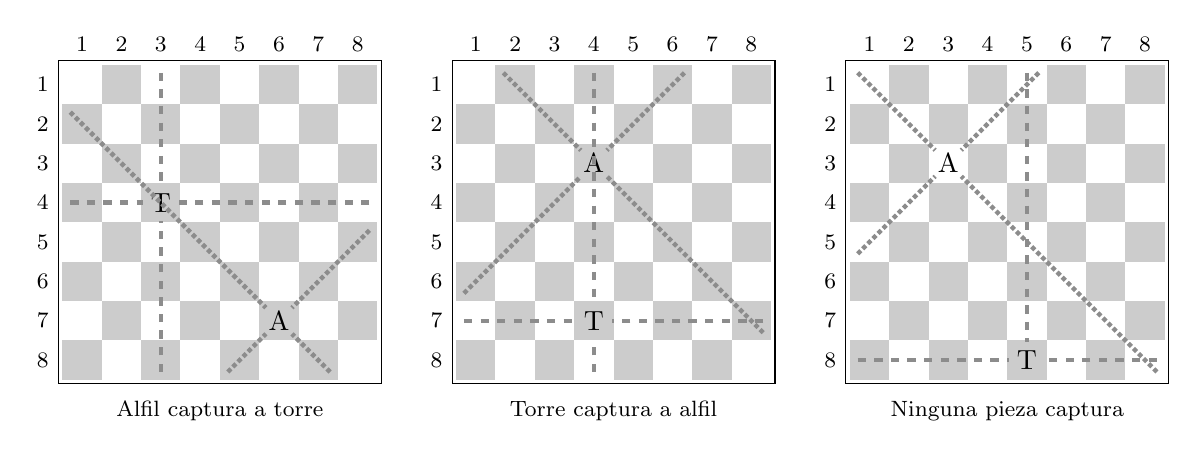
\begin{tikzpicture}[scale=.5, yscale=-1]
  \begin{scope}
    \tablero
    \node[pieza] (alfil) at (6, 7) {A};
    \node[pieza] (torre) at (3, 4) {T};
    \draw[ma] (1 - \d, 2 - \d) -- (alfil);
    \draw[ma] (5 - \d, 8 + \d) -- (alfil);
    \draw[ma] (8 + \d, 5 - \d) -- (alfil);
    \draw[ma] (7 + \d, 8 + \d) -- (alfil);
    \draw[mt] (3     , 1 - \d) -- (torre);
    \draw[mt] (3     , 8 + \d) -- (torre);
    \draw[mt] (1 - \d, 4     ) -- (torre);
    \draw[mt] (8 + \d, 4     ) -- (torre);
    \node at (4.5, 9.3) {\footnotesize Alfil captura a torre};
  \end{scope}
  \begin{scope}[xshift=10cm]
    \tablero
    \node[pieza] (alfil) at (4, 3) {A};
    \node[pieza] (torre) at (4, 7) {T};
    \draw[ma] (2 - \d, 1 - \d) -- (alfil);
    \draw[ma] (1 - \d, 6 + \d) -- (alfil);
    \draw[ma] (6 + \d, 1 - \d) -- (alfil);
    \draw[ma] (8 + \d, 7 + \d) -- (alfil);
    \draw[mt] (4     , 1 - \d) -- (torre);
    \draw[mt] (4     , 8 + \d) -- (torre);
    \draw[mt] (1 - \d, 7     ) -- (torre);
    \draw[mt] (8 + \d, 7     ) -- (torre);
    \node at (4.5, 9.3) {\footnotesize Torre captura a alfil};
  \end{scope}
  \begin{scope}[xshift=20cm]
    \tablero
    \node[pieza] (alfil) at (3, 3) {A};
    \node[pieza] (torre) at (5, 8) {T};
    \draw[ma] (1 - \d, 1 - \d) -- (alfil);
    \draw[ma] (1 - \d, 5 + \d) -- (alfil);
    \draw[ma] (5 + \d, 1 - \d) -- (alfil);
    \draw[ma] (8 + \d, 8 + \d) -- (alfil);
    \draw[mt] (5     , 1 - \d) -- (torre);
    %\draw[mt] (5     , 8 + \d) -- (torre);
    \draw[mt] (8 + \d, 8     ) -- (torre);
    \draw[mt] (1 - \d, 8     ) -- (torre);
    \node at (4.5, 9.3) {\footnotesize Ninguna pieza captura};
  \end{scope}
\end{tikzpicture}

